
%% bare_conf.tex
%% V1.4b
%% 2015/08/26
%% by Michael Shell
%% See:
%% http://www.michaelshell.org/
%% for current contact information.
%%
%% This is a skeleton file demonstrating the use of IEEEtran.cls
%% (requires IEEEtran.cls version 1.8b or later) with an IEEE
%% conference paper.
%%
%% Support sites:
%% http://www.michaelshell.org/tex/ieeetran/
%% http://www.ctan.org/pkg/ieeetran
%% and
%% http://www.ieee.org/

%%*************************************************************************
%% Legal Notice:
%% This code is offered as-is without any warranty either expressed or
%% implied; without even the implied warranty of MERCHANTABILITY or
%% FITNESS FOR A PARTICULAR PURPOSE! 
%% User assumes all risk.
%% In no event shall the IEEE or any contributor to this code be liable for
%% any damages or losses, including, but not limited to, incidental,
%% consequential, or any other damages, resulting from the use or misuse
%% of any information contained here.
%%
%% All comments are the opinions of their respective authors and are not
%% necessarily endorsed by the IEEE.
%%
%% This work is distributed under the LaTeX Project Public License (LPPL)
%% ( http://www.latex-project.org/ ) version 1.3, and may be freely used,
%% distributed and modified. A copy of the LPPL, version 1.3, is included
%% in the base LaTeX documentation of all distributions of LaTeX released
%% 2003/12/01 or later.
%% Retain all contribution notices and credits.
%% ** Modified files should be clearly indicated as such, including  **
%% ** renaming them and changing author support contact information. **
%%*************************************************************************


% *** Authors should verify (and, if needed, correct) their LaTeX system  ***
% *** with the testflow diagnostic prior to trusting their LaTeX platform ***
% *** with production work. The IEEE's font choices and paper sizes can   ***
% *** trigger bugs that do not appear when using other class files.       ***                          ***
% The testflow support page is at:
% http://www.michaelshell.org/tex/testflow/



\documentclass[conference]{IEEEtran}
% Some Computer Society conferences also require the compsoc mode option,
% but others use the standard conference format.
%
% If IEEEtran.cls has not been installed into the LaTeX system files,
% manually specify the path to it like:
% \documentclass[conference]{../sty/IEEEtran}





% Some very useful LaTeX packages include:
% (uncomment the ones you want to load)


% *** MISC UTILITY PACKAGES ***
%
%\usepackage{ifpdf}
% Heiko Oberdiek's ifpdf.sty is very useful if you need conditional
% compilation based on whether the output is pdf or dvi.
% usage:
% \ifpdf
%   % pdf code
% \else
%   % dvi code
% \fi
% The latest version of ifpdf.sty can be obtained from:
% http://www.ctan.org/pkg/ifpdf
% Also, note that IEEEtran.cls V1.7 and later provides a builtin
% \ifCLASSINFOpdf conditional that works the same way.
% When switching from latex to pdflatex and vice-versa, the compiler may
% have to be run twice to clear warning/error messages.






% *** CITATION PACKAGES ***
%
\usepackage{cite}
% cite.sty was written by Donald Arseneau
% V1.6 and later of IEEEtran pre-defines the format of the cite.sty package
% \cite{} output to follow that of the IEEE. Loading the cite package will
% result in citation numbers being automatically sorted and properly
% "compressed/ranged". e.g., [1], [9], [2], [7], [5], [6] without using
% cite.sty will become [1], [2], [5]--[7], [9] using cite.sty. cite.sty's
% \cite will automatically add leading space, if needed. Use cite.sty's
% noadjust option (cite.sty V3.8 and later) if you want to turn this off
% such as if a citation ever needs to be enclosed in parenthesis.
% cite.sty is already installed on most LaTeX systems. Be sure and use
% version 5.0 (2009-03-20) and later if using hyperref.sty.
% The latest version can be obtained at:
% http://www.ctan.org/pkg/cite
% The documentation is contained in the cite.sty file itself.






% *** GRAPHICS RELATED PACKAGES ***
%
\ifCLASSINFOpdf
% \usepackage[pdftex]{graphicx}
% declare the path(s) where your graphic files are
% \graphicspath{{../pdf/}{../jpeg/}}
% and their extensions so you won't have to specify these with
% every instance of \includegraphics
% \DeclareGraphicsExtensions{.pdf,.jpeg,.png}
\else
% or other class option (dvipsone, dvipdf, if not using dvips). graphicx
% will default to the driver specified in the system graphics.cfg if no
% driver is specified.
% \usepackage[dvips]{graphicx}
% declare the path(s) where your graphic files are
% \graphicspath{{../eps/}}
% and their extensions so you won't have to specify these with
% every instance of \includegraphics
% \DeclareGraphicsExtensions{.eps}
\fi
% graphicx was written by David Carlisle and Sebastian Rahtz. It is
% required if you want graphics, photos, etc. graphicx.sty is already
% installed on most LaTeX systems. The latest version and documentation
% can be obtained at: 
% http://www.ctan.org/pkg/graphicx
% Another good source of documentation is "Using Imported Graphics in
% LaTeX2e" by Keith Reckdahl which can be found at:
% http://www.ctan.org/pkg/epslatex
%
% latex, and pdflatex in dvi mode, support graphics in encapsulated
% postscript (.eps) format. pdflatex in pdf mode supports graphics
% in .pdf, .jpeg, .png and .mps (metapost) formats. Users should ensure
% that all non-photo figures use a vector format (.eps, .pdf, .mps) and
% not a bitmapped formats (.jpeg, .png). The IEEE frowns on bitmapped formats
% which can result in "jaggedy"/blurry rendering of lines and letters as
% well as large increases in file sizes.
%
% You can find documentation about the pdfTeX application at:
% http://www.tug.org/applications/pdftex





% *** MATH PACKAGES ***
%
%\usepackage{amsmath}
% A popular package from the American Mathematical Society that provides
% many useful and powerful commands for dealing with mathematics.
%
% Note that the amsmath package sets \interdisplaylinepenalty to 10000
% thus preventing page breaks from occurring within multiline equations. Use:
%\interdisplaylinepenalty=2500
% after loading amsmath to restore such page breaks as IEEEtran.cls normally
% does. amsmath.sty is already installed on most LaTeX systems. The latest
% version and documentation can be obtained at:
% http://www.ctan.org/pkg/amsmath





% *** SPECIALIZED LIST PACKAGES ***
%
%\usepackage{algorithmic}
% algorithmic.sty was written by Peter Williams and Rogerio Brito.
% This package provides an algorithmic environment fo describing algorithms.
% You can use the algorithmic environment in-text or within a figure
% environment to provide for a floating algorithm. Do NOT use the algorithm
% floating environment provided by algorithm.sty (by the same authors) or
% algorithm2e.sty (by Christophe Fiorio) as the IEEE does not use dedicated
% algorithm float types and packages that provide these will not provide
% correct IEEE style captions. The latest version and documentation of
% algorithmic.sty can be obtained at:
% http://www.ctan.org/pkg/algorithms
% Also of interest may be the (relatively newer and more customizable)
% algorithmicx.sty package by Szasz Janos:
% http://www.ctan.org/pkg/algorithmicx




% *** ALIGNMENT PACKAGES ***
%
%\usepackage{array}
% Frank Mittelbach's and David Carlisle's array.sty patches and improves
% the standard LaTeX2e array and tabular environments to provide better
% appearance and additional user controls. As the default LaTeX2e table
% generation code is lacking to the point of almost being broken with
% respect to the quality of the end results, all users are strongly
% advised to use an enhanced (at the very least that provided by array.sty)
% set of table tools. array.sty is already installed on most systems. The
% latest version and documentation can be obtained at:
% http://www.ctan.org/pkg/array


% IEEEtran contains the IEEEeqnarray family of commands that can be used to
% generate multiline equations as well as matrices, tables, etc., of high
% quality.




% *** SUBFIGURE PACKAGES ***
\ifCLASSOPTIONcompsoc
  \usepackage[caption=false,font=normalsize,labelfont=sf,textfont=sf]{subfig}
\else
  \usepackage[caption=false,font=footnotesize]{subfig}
\fi
% subfig.sty, written by Steven Douglas Cochran, is the modern replacement
% for subfigure.sty, the latter of which is no longer maintained and is
% incompatible with some LaTeX packages including fixltx2e. However,
% subfig.sty requires and automatically loads Axel Sommerfeldt's caption.sty
% which will override IEEEtran.cls' handling of captions and this will result
% in non-IEEE style figure/table captions. To prevent this problem, be sure
% and invoke subfig.sty's "caption=false" package option (available since
% subfig.sty version 1.3, 2005/06/28) as this is will preserve IEEEtran.cls
% handling of captions.
% Note that the Computer Society format requires a larger sans serif font
% than the serif footnote size font used in traditional IEEE formatting
% and thus the need to invoke different subfig.sty package options depending
% on whether compsoc mode has been enabled.
%
% The latest version and documentation of subfig.sty can be obtained at:
% http://www.ctan.org/pkg/subfig




% *** FLOAT PACKAGES ***
%
%\usepackage{fixltx2e}
% fixltx2e, the successor to the earlier fix2col.sty, was written by
% Frank Mittelbach and David Carlisle. This package corrects a few problems
% in the LaTeX2e kernel, the most notable of which is that in current
% LaTeX2e releases, the ordering of single and double column floats is not
% guaranteed to be preserved. Thus, an unpatched LaTeX2e can allow a
% single column figure to be placed prior to an earlier double column
% figure.
% Be aware that LaTeX2e kernels dated 2015 and later have fixltx2e.sty's
% corrections already built into the system in which case a warning will
% be issued if an attempt is made to load fixltx2e.sty as it is no longer
% needed.
% The latest version and documentation can be found at:
% http://www.ctan.org/pkg/fixltx2e


\usepackage{stfloats}
% stfloats.sty was written by Sigitas Tolusis. This package gives LaTeX2e
% the ability to do double column floats at the bottom of the page as well
% as the top. (e.g., "\begin{figure*}[!b]" is not normally possible in
% LaTeX2e). It also provides a command:
%\fnbelowfloat
% to enable the placement of footnotes below bottom floats (the standard
% LaTeX2e kernel puts them above bottom floats). This is an invasive package
% which rewrites many portions of the LaTeX2e float routines. It may not work
% with other packages that modify the LaTeX2e float routines. The latest
% version and documentation can be obtained at:
% http://www.ctan.org/pkg/stfloats
% Do not use the stfloats baselinefloat ability as the IEEE does not allow
% \baselineskip to stretch. Authors submitting work to the IEEE should note
% that the IEEE rarely uses double column equations and that authors should try
% to avoid such use. Do not be tempted to use the cuted.sty or midfloat.sty
% packages (also by Sigitas Tolusis) as the IEEE does not format its papers in
% such ways.
% Do not attempt to use stfloats with fixltx2e as they are incompatible.
% Instead, use Morten Hogholm'a dblfloatfix which combines the features
% of both fixltx2e and stfloats:
%
% \usepackage{dblfloatfix}
% The latest version can be found at:
% http://www.ctan.org/pkg/dblfloatfix




% *** PDF, URL AND HYPERLINK PACKAGES ***
%
%\usepackage{url}
% url.sty was written by Donald Arseneau. It provides better support for
% handling and breaking URLs. url.sty is already installed on most LaTeX
% systems. The latest version and documentation can be obtained at:
% http://www.ctan.org/pkg/url
% Basically, \url{my_url_here}.




% *** Do not adjust lengths that control margins, column widths, etc. ***
% *** Do not use packages that alter fonts (such as pslatex).         ***
% There should be no need to do such things with IEEEtran.cls V1.6 and later.
% (Unless specifically asked to do so by the journal or conference you plan
% to submit to, of course. )

\usepackage{booktabs} % For formal tables
\usepackage{multirow}
\usepackage{algorithm}
\usepackage[noend]{algpseudocode}
\usepackage[pdftex]{graphicx}
\usepackage[T1,hyphens]{url}
%\usepackage[colorlinks,urlcolor=blue]{hyperref}
\usepackage[]{hyperref}
\usepackage[usenames, dvipsnames]{color}
%\usepackage{graphicx,times}
%\usepackage{subfigure}         
%\usepackage{natbib}
%\usepackage{amssymb,amsmath}
%\usepackage{geometry}

\graphicspath{{./figures/}}
\algrenewcommand\textproc{}

%\algsetup{linenosize=\small}

% correct bad hyphenation here
\hyphenation{op-tical net-works semi-conduc-tor}


\begin{document}
%
% paper title
% Titles are generally capitalized except for words such as a, an, and, as,
% at, but, by, for, in, nor, of, on, or, the, to and up, which are usually
% not capitalized unless they are the first or last word of the title.
% Linebreaks \\ can be used within to get better formatting as desired.
% Do not put math or special symbols in the title.
%\title{Breadth First Search on FPGAs: A Pipelined Execution Approach}
\title{Resilient neural network training for accelerators with computing errors}

% author names and affiliations
% use a multiple column layout for up to three different
% affiliations
\author{\IEEEauthorblockN{Dawen Xu\textsuperscript{1,2}, Kouzi Xing\textsuperscript{1}, Cheng Liu\textsuperscript{2}, Ying Wang\textsuperscript{2}, Yulin Dai\textsuperscript{1}, Long Cheng\textsuperscript{3}, Huawei Li\textsuperscript{2}, Lei Zhang\textsuperscript{2}}
\IEEEauthorblockA{\textsuperscript{1}HeFei University of Technology, HeFei, China\\
\textsuperscript{2}Institute of Computing Technology, Chinese Academy of Sciences, BeiJing, China\\
\textsuperscript{3}University College Dublin\\
Email: liucheng@ict.ac.cn}
%\and
%\IEEEauthorblockN{Homer Simpson}
%\IEEEauthorblockA{Twentieth Century Fox\\
%Springfield, USA\\
%Email: homer@thesimpsons.com}
%\and
%\IEEEauthorblockN{James Kirk\\ and Montgomery Scott}
%\IEEEauthorblockA{Starfleet Academy\\
%San Francisco, California 96678--2391\\
%Telephone: (800) 555--1212\\
%Fax: (888) 555--1212}
}

% conference papers do not typically use \thanks and this command
% is locked out in conference mode. If really needed, such as for
% the acknowledgment of grants, issue a \IEEEoverridecommandlockouts
% after \documentclass

% for over three affiliations, or if they all won't fit within the width
% of the page, use this alternative format:
% 
%\author{\IEEEauthorblockN{Michael Shell\IEEEauthorrefmark{1},
%Homer Simpson\IEEEauthorrefmark{2},
%James Kirk\IEEEauthorrefmark{3}, 
%Montgomery Scott\IEEEauthorrefmark{3} and
%Eldon Tyrell\IEEEauthorrefmark{4}}
%\IEEEauthorblockA{\IEEEauthorrefmark{1}School of Electrical and Computer Engineering\\
%Georgia Institute of Technology,
%Atlanta, Georgia 30332--0250\\ Email: see http://www.michaelshell.org/contact.html}
%\IEEEauthorblockA{\IEEEauthorrefmark{2}Twentieth Century Fox, Springfield, USA\\
%Email: homer@thesimpsons.com}
%\IEEEauthorblockA{\IEEEauthorrefmark{3}Starfleet Academy, San Francisco, California 96678-2391\\
%Telephone: (800) 555--1212, Fax: (888) 555--1212}
%\IEEEauthorblockA{\IEEEauthorrefmark{4}Tyrell Inc., 123 Replicant Street, Los Angeles, California 90210--4321}}




% use for special paper notices
%\IEEEspecialpapernotice{(Invited Paper)}




% make the title area
\maketitle

% As a general rule, do not put math, special symbols or citations
% in the abstract
\begin{abstract}
With the advancements of neural networks, customized accelerators 
are increasingly adopted in massive AI applications. To gain higher energy 
efficiency or performance, many hardware design optimizations 
such as near-threshold logic or overclocking can be utilized. 
In these cases, computing errors may happen and the computing errors are difficult to be captured 
by conventional training on general purposed processors (GPPs). 
Applying the offline trained neural network models to the accelerators 
with errors directly may lead to considerable prediction
accuracy loss.

To address this problem, we explore the resilience of
neural network models and relax the accelerator design constraints 
to enable aggressive design options. First of all, we 
propose to train the neural network models
using the accelerators' forward computing results 
such that the models can learn both the data and the computing
errors. In addition, we observe that some of the neural network layers
are more sensitive to the computing errors. With this observation,
we schedule the most sensitive layer to the attached GPP 
to reduce the negative influence of the computing errors. 
According to the experiments, the neural network models 
obtained from the proposed training outperform the original
models significantly when the CNN accelerators are
affected by computing errors.
\end{abstract}

% no keywords


% For peer review papers, you can put extra information on the cover
% page as needed:
% \ifCLASSOPTIONpeerreview
% \begin{center} \bfseries EDICS Category: 3-BBND \end{center}
% \fi
%
% For peerreview papers, this IEEEtran command inserts a page break and
% creates the second title. It will be ignored for other modes.
\IEEEpeerreviewmaketitle

\section{Introduction} \label{sec:intro}
Inspired by the widespread adoption of neural networks in massive fields such as image classification, 
video surveillance, speech recognition, and robot vision, neural network accelerators 
\cite{Zhang2015_9,Qiu2016_10,deepburing_12,DiCecco_4,Zeng2018_18} 
are increasingly explored and deployed to improve the computing performance and energy efficiency.
Unlike generic applications, neural networks usually involve redundancy and are known to be 
fault tolerant\cite{Reagen2016}. By taking advantage of this feature, many neural network accelerator optimizations 
such as neural network pruning and low-precision quantization can be utilized to improve 
performance and energy efficiency notably with minor inference accuracy penalty\cite{Han2016DeepCC}. 

In line with these optimizations, we opt to relax the design constraints of 
the neural network accelerators, which provides a unique way to achieve notable 
improvements on performance or energy efficiency with small inference accuracy loss. 
For generic hardware design, strict design constraint is typically required to 
guarantee correct computing under even the most severe environments. On the contrast, 
neural network accelerators are more resilient and less sensitive to computing 
errors incurred by timing violations. Given relaxed design constraints, many 
aggressive hardware optimization techniques can be applied with computing errors. 
For instance, emerging techniques such as  near-threshold voltage regime\cite{RG2010NT} 
and subthreshold digital logic design\cite{BH2005,B2006} promise high energy efficiency 
but suffer instability\cite{Pu2010NT}. Conventional neural network accelerator 
can be pushed to operate at higher clock frequency with timing violations
\cite{overclock_3,Paceline_15}. At the fab level, design rules may also 
be aggressively pushed to reduce the expense. 

Motivated by the great advantages of relaxed design constraints,
we further explore the use of neural network resilience for more 
effective design trade-offs. When there are timing violations
and computing errors in the accelerator, the unmodified neural networks 
executed on the accelerators during inference is different 
from that computed on GPPs during the training, which may cause clear 
prediction accuracy loss. Instead of deploying the unmodified neural 
network models on the accelerators directly, we borrow the retraining 
idea from prior neural network quantization work \cite{Hwang2014_17,Matthieu2014_8} 
and have the deep neural network models to learn and tolerate the computing errors.  
Basically, we have the forward computing performed on the accelerator and 
then transfer the computing results to the host processor for 
backward propagation. With this approach, both application data and computing 
errors are learned and incorporated in the neural network models.  
Meanwhile, we define a set of standard interfaces to make it convenient 
to integrate general CNN accelerators into the retraining framework. 

In addition, we notice that some of the neural network layers are more sensitive to the 
computing errors and the sensitive layers dramatically limit the usefulness of the retraining. 
Thus, we schedule the most sensitive layer which is usually the last 
layer of the neural networks to host processors to reduce the negative influence 
of the computing errors. With both the retraining and sensitive layer protection, 
the neural networks become more resilient to the computing errors caused by 
the aggressive design options such as near-threshold logic or overclocking.
Compared to the original neural networks, the prediction accuracy of top-1 and top-5 
improves by 22.8\% and 9.89\% on average. The contributions of this work are 
summarized as follows.

\begin{itemize}
	\item We propose to improve the fault-tolerance of neural networks and make use of it to relax 
		the accelerator design constraints for higher performance or energy efficiency.

	\item We propose a neural network training framework to obtain resilient neural network models. 
		By integrating accelerator into conventional training, we have the computing errors 
		learned with the application data. By protecting the layer with most large errors, 
		we can further improve the resilience of the neural networks and pose more 
		opportunities to hardware optimizations.

	\item With comprehensive experiments, we show that the proposed training framework 
		could enhance the prediction accuracy of neural networks significantly 
		when the accelerators run with computing errors incurred by either 
		overclocking or lower voltage.
\end{itemize}
The paper is organized as follows. Section II analyzes the influence of 
the CNN accelerator computing errors on the neural network prediction accuracy. 
Section III presents the proposed training for neural networks executed on accelerators with computing errors.
Section IV demonstrate the use of the training on accelerators with overclocking and generic computing errors. 
Section V briefs the related work and Section VI draws the conclusion. 



%\section{Motivation} \label{sec:motivation}
Clock frequency determines the accelerator operation speed 
and directly affects the performance. Accordingly, it also has influence on the 
neural network runtime and energy efficiency. In this section, we take 
an open-sourced CNN accelerator named PipeCNN \cite{pipecnn_2} as an example and analyze its 
influence on the neural network performance and energy efficiency.

The accelerator is implemented on KCU1500 and attached to a desktop computer with 
Intel i7-6700@3.40GHz. The basic convolution structure is shown in Fig \ref{fig:cnn-arch}. The largest computing 
array that can be accommodated by the FPGA device consists of 16 dot production units. 
Each dot production unit allows parallel processing of two 8-data vectors.
The accelerator consumes over 11\% LUT of the FPGA device. The optimized clock frequency 
according to the SDAccel compilation is 200 MHz. 

\begin{figure}
	\center{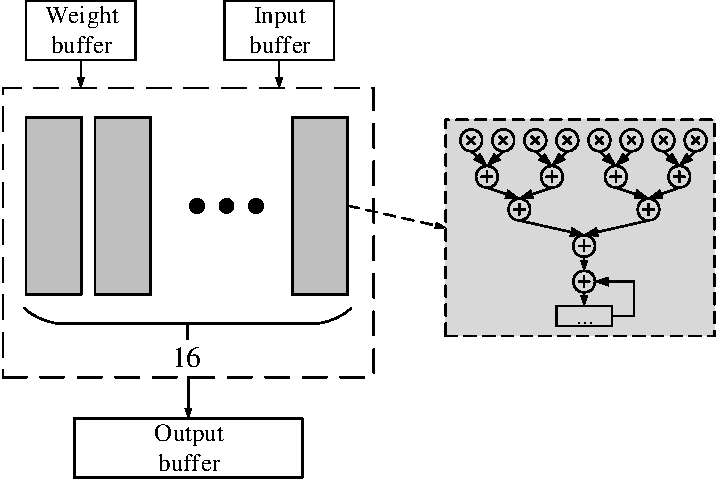
\includegraphics[width=0.75\linewidth]{accelerator}}
    \caption{Baseline CNN accelerator architecture.}
\label{fig:cnn-arch}
\vspace{-1em}
\end{figure}


In order to evaluate the influence of clock 
frequency, we further set the clock to 50 MHz, 100 MHz, and 150 MHz respectively.
A set of neural networks including LeNet, AlexNet, VGG-16 and VGG-19 are used as the benchmark.
Normalized performance the neural network benchmark executed on the accelerators are 
shown in Fig \ref{fig:computing-bound}. It can be found that the 
overall performance of the neural network benchmark
almost increases proportional to the clock frequency. For the larger neural networks, 
the processing remains the computing bound and high frequency design is highly demanded.

\begin{figure}
	\center{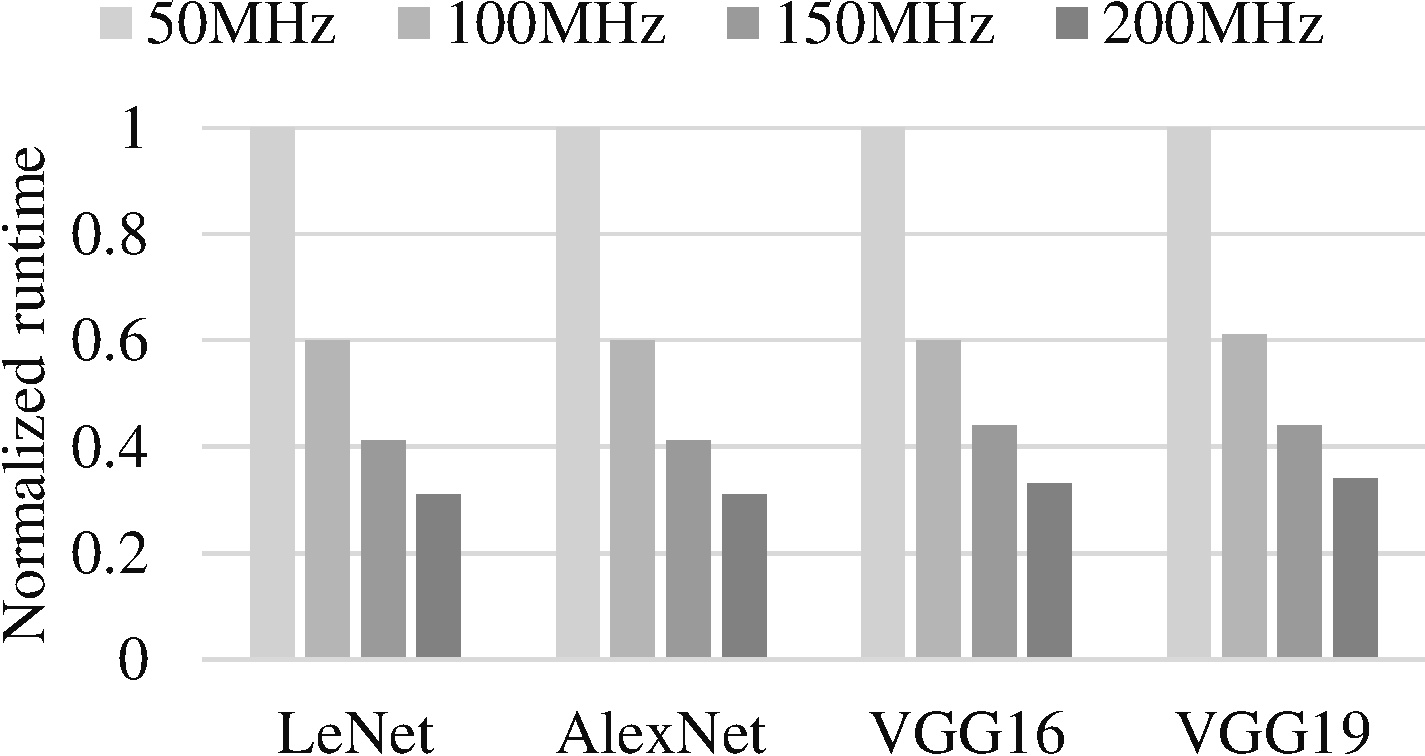
\includegraphics[width=0.75\linewidth]{relative_time}}
    \caption{Normalized performance of neural networks executed on CNN accelerators with different clock frequency.}
\label{fig:computing-bound}
\vspace{-1em}
\end{figure}

In addition, we also obtain the power consumption from SDAccel report. 
The power estimation setup assumes xxxx. Given the power consumption and the performance, 
we calcualted the energy delay product which can be used as an energy efficiency metric.
The energy efficiency is presented in Fig \ref{fig:edp}.
\begin{figure}
	\center{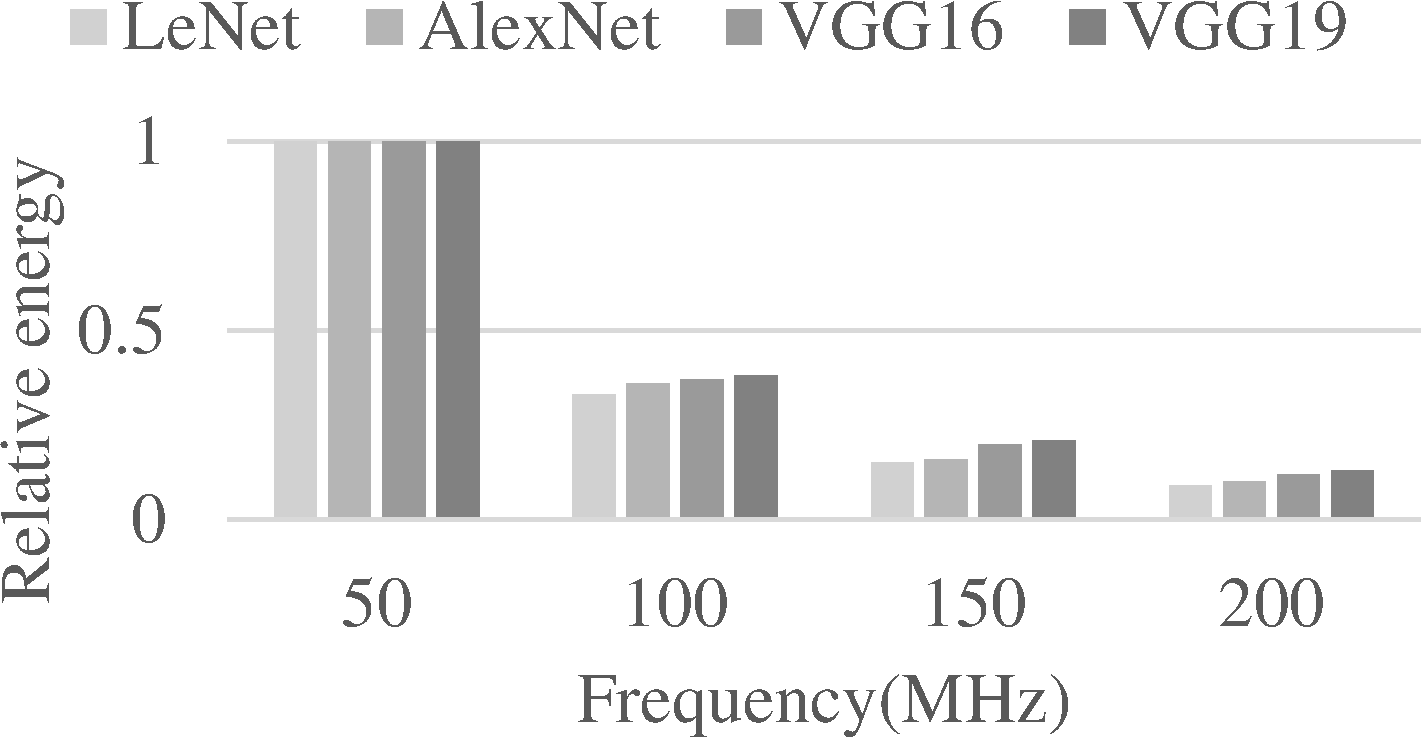
\includegraphics[width=0.75\linewidth]{relative_energy}}
    \caption{Normalized energy-delay product of neural networks executed on CNN accelerators with different clock frequency.}
\label{fig:edp}
\vspace{-1em}
\end{figure}

According to the above experiments, it can be conclcuded that higher clock frequency 
can be beneficial to both the neural network performance and energy efficiency. The 
potential performance and energy efficiency improvement indicates that it is 
worthwhile to boosting the clock of FPGA based CNN accelerators with some minor 
overhead. Detailed overclocking on CNN accelerators will be investigated in 
detail in the rest part of this paper. 

\section{Resilient training framework} \label{sec:framework}
Resilient neural networks allow significant performance or 
energy efficiency improvement with little prediction accuracy penalty 
by relaxing the neural network accelerator design constraints. 
This motivates us to obtain more resilient neural networks 
for advantageous accelerator design trade-offs. 
A resilient neural network training framework will be 
detailed in this section. 

\subsection{Overall training framework}
For the problem that the computing error patterns are 
difficult to be captured in training with GPPs, 
we have the accelerators with computing errors integrated into 
the training process. Forward processing influenced by 
the accelerator computing errors is used in training directly 
such that computing error patterns and application data are 
reflected in the neural network models. For the problem that 
some of the layers are affected more than the others, 
we take these layers as critical layers and opt to 
protect the layers from being affected by computing errors. 
With reasonable performance penalty, we can improve the 
overall neural network resilience. 

Following this idea, the overall training framework is depicted in Figure \ref{fig:retrain}. 
Instead of training on GPPs, it has the majority of forward computing performed on the 
accelerators with computing errors while the rest of the training remains on GPPs.
Note that the critical layers should be executed on reliable hardware 
while GPP is one of the options. There are many different approaches 
that can be used to relax the design constraints.
Although they may cause distinct computing errors, they can be fitted to the 
same training framework.

\begin{figure}
        \center{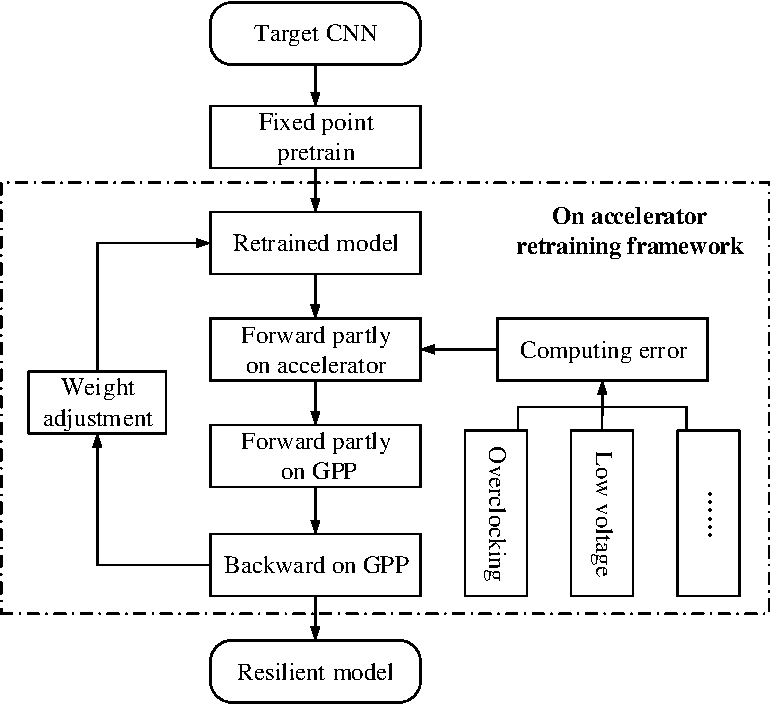
\includegraphics[width=0.85\linewidth]{on_accelerator_retrain_pocess}}
        \caption{Resilient neural network training framework}
        \label{fig:retrain}
        \vspace{-1em}
\end{figure}

\subsection{CNN accelerator abstraction and modification}
As illustrated in the above section, the forward propagation will 
mostly be executed on the CNN accelerator while 
the rest part runs on GPPs. Essentially, the framework targets at a 
heterogeneous computing architecture and frequent 
communication between the accelerator and the GPPs are expected. 
In order to fit various CNN accelerators within the same training framework,
we abstract the CNN accelerators with a high-level interface
which makes the accelerators near transparent to the training framework.
To facilitate the data communication between the forward propagation
and the rest of the training framework, we define a high-level
interface which consists of 7 functions as listed inTable \ref{tab:api}.
%Function 1 is used to launch the CNN accelerator from host. 
%Function 2 and 3 are used to transfer data between the host memory and the device memory during 
%the training. As the forward propagation on the CNN accelerators is usually fixed point 
%and the back propagation on GPPs is floating point, data type converting between fixed point 
%and floating point is required. Function 4 and 5 can be used for this purpose. 
%Function 1 to 5 are required for all the accelerators. 
%Function 6 and 7 are only used for accelerators that compute on reorganized data\cite{pipecnn_2,deepburing_12}. 
With the interface functions, general CNN accelerators can be conveniently
referenced and used in the proposed on-accelerator training framework.
\begin{table*}
	\
        \centering
        \vspace{-0.3em}
        \caption{High-level interface to integrate general CNN accelerators with Caffe}
        \label{tab:api}
        \vspace{-0.3em}
        \begin{tabular}{c|l|l}
                \toprule
                ID & Function Name & Description  \\
                \midrule
                1 & launchAccelerator() & It configures the CNN accelerator and launches it from host CPU. \\
		\midrule
                2 & dataToFPGA(weight, input, wgtDevAddr, inDevAddr) & It transfers both the input data and weight to the FPGA device memory. \\
		\midrule
		3 & dataFromFPGA(outputDevAddr, output) & \shortstack[l]{It transfers intermediate data from FPGA device memory to host memory.} \\
		\midrule
		4 & convertIntToFloat(int iData, float fData) & It converts the fixed-point point to float for back propagation processing. \\
		\midrule
		5 & convertFloatToInt(float fData,  int iData) & \shortstack[l]{It converts the floating-point input and weight to fixed point for forward processing.} \\
		\midrule
		6 & dataLayoutReorder(data, reorderedData) & \shortstack[l]{It reorders the data layout for more efficient accelerator execution.} \\
		\midrule
		7 & dataLayoutRecover(reorderedData, data) & It reorders the output data back to the default format for Caffe back propagation. \\
                \bottomrule
        \end{tabular}
        \vspace{-1em}
\end{table*}

In this work, we have the CNN accelerator implemented on Xilinx FPGAs as a case study. 
With Xilinx SDAccel, we can wrap the accelerators with OpenCL API while the accelerators 
can either be developed with OpenCL, HLS or RTL. On top of the OpenCL API, the proposed 
high-level interface can be implemented. Meanwhile, we use Caffe, a C++ based 
deep learning framework, to construct the on-accelerator training framework. With 
both parts developed with C family languages, they can be integrated conveniently. 

%In this work, we have the CNN accelerator implemented on FPGAs.
%Figure 4 depicts the implementation of the training framework on a hybrid 
%CPU-FPGA architecture. In this work, we use Xilinx KCU1500 as the FPGA board 
%and put it on a standard desktop computer. CPU is the controller and it reconfigures 
%the accelerator for a specific CNN structure. In each training iteration, CPU launches 
%the CNN accelerator to perform the forward propagation from bottom layer to top layer. 
%CPU does the backward propagation from top layer to bottom layer. Weights and the image 
%data are initially stored in host memory. It will be transferred to FPGA offchip memory 
%for forward propagation through PCI-E. Similarly, the output data will be transferred 
%from FPGA off-chip memory back to host memory after forward propagation. Because of the 
%OpenCL based API wrapper in SDAccel, the CNN accelerator’s interface can be easily 
%exposed to Caffe for referring to the forward propagation result. 

\begin{figure}
        \center{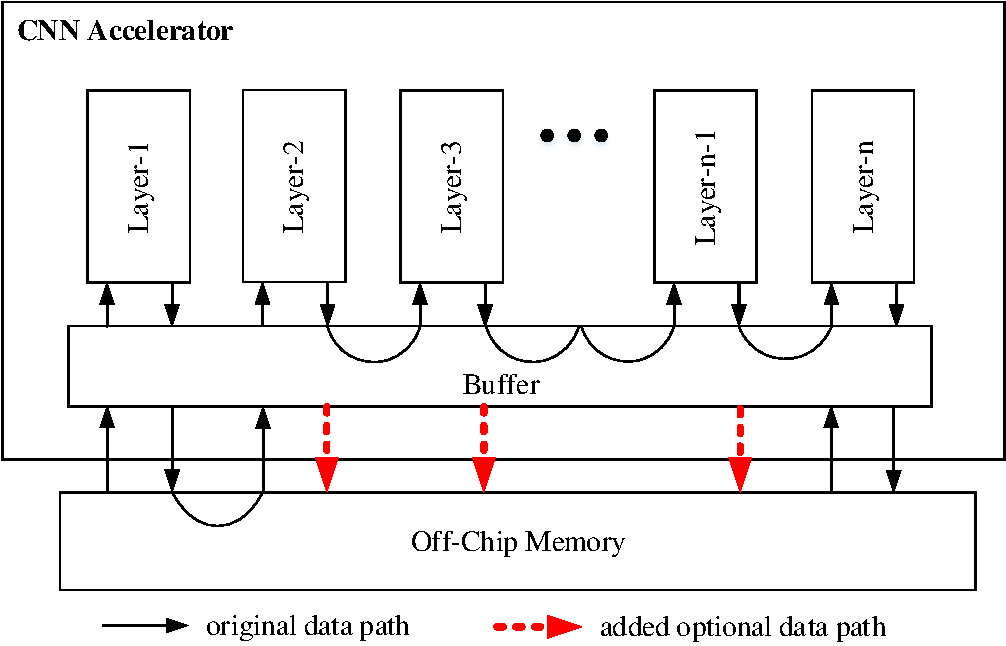
\includegraphics[width=0.85\linewidth]{change_of_accelerator}}
        \caption{Modification of the CNN accelerator data path. It essentially
ensures the feature map of each neural network layer to have an optional data path
to external memory for back propagation in training.}
        \label{fig:change_of_accelerator}
        \vspace{-1em}
\end{figure}

On top of the high-level interface, the CNN accelerator also needs 
minor modification to enable the on-accelerator training. 
The training requires the feature map of each neural 
network layer for backward propagation. However, many of the accelerators 
are intensively optimized for inference only and some of the layers' output 
are fully buffered in on-chip memory to reduce the external memory access. 
Thereby, the accelerator should provide an optional data path such that 
intermediate output data can be written to external memory at request.
As shown in Figure \ref{fig:change_of_accelerator}, the output of each layer 
will be transferred to memory using the added data path 
when the accelerator is used for training. The write back data path 
can be switched off during inference. 

\subsection{Critical neural network layer protection}
In order to improve the overall neural network resilience, we opt to 
protect the critical network layers to alleviate the resilience 
bottleneck. The protection is essentially 
to have the critical layers executed on reliable computing infrastructures 
and the exact protection method depends on the target hardware platform.
We may either schedule the critical layers to the GPPs or switch the accelerator 
to reliable mode during the execution of the critical layers.
With this approach, the overall network can tolerate 
more computing errors. 

To decide the critical layers of the neural networks, we formulate the 
critical layer selection scheme. Suppose the neural network layers include 
$N$ layers and each layer is represented as $L_i$ where $i \in {0, 1, 2, ..., N-1}$.
Then we evaluate the prediction accuracy loss of the neural network 
that have one layer protected on accelerators with computing errors.
When the $i$th layer is protected, the loss is $loss_i$.
Then the most critical layer is the layer that leads to the most 
accuracy loss i.e. $c \in \{k|loss_k = max(loss_i), i \in \{0, 1, ..., N-1\}\}$.

The above formulated approach requires large amount of evaluation of 
different layers of the neural network. Instead, we use the actual 
computing errors as the critical layer selection metric. We set an 
error threshold $T$ and assume 8bit integers are used. 
When the error equals to 0, the computing results are correct. 
When the error is larger than $T$, the results are assumed to be large errors.
When the computing results are wrong but smaller than $T$, the results are considered 
as moderate errors. The layers that include the largest portion of large errors 
are taken as the critical layers.

In addition, scheduling the neural network layers executed 
on the accelerator to GPPs has performance penalty due to the 
computing efficiency gap. As the accelerators are usually 
orders of magnitudes faster than the GPPs for neural network 
processing especially large convolution layers, we can focus on 
the last few small layers to ensure negligible performance 
loss. This constrain greatly reduces the search space
of the critical layers. 



\section{Experiments} \label{sec:casestudy}
In this section, we evaluate the proposed resilient neural network training 
framework for accelerators with computing errors. The errors can be caused by 
various relaxed design constraints and we use random computing errors in 
the experiments for general analysis. Then we use overclocking on FPGA based 
CNN accelerators as the case study and demonstrate the usefulness of the 
proposed resilient training on realistic system.

\subsection{Experiment setup}
We experiment on 8bit fixed-point PipeCNN \cite{pipecnn_2} accelerators on Xilinx KCU1500.
The FPGA board is attached to Intel(R) Core(TM) i7-6700 CPU @3.40GHz with 32GB memory.
To simulate general hardware errors caused by relaxed design constraints, we 
inject random bit errors to input/output data including 
input/intermediate/output features and weights as well as 
hidden layer status of neural networks. The error injection is measured with 
bit error rate (BER) which is also utilized in xxx. Compared to xxx,
we also have random errors injected to the internal computing results. 
To evaluate the training, we take three representative convolution 
neural networks including AlexNet, VGG-16 and VGG-19 as the benchmark. 
The neural network benchmark is summarized in Table \ref{tab:CNN-table}. 
The analysis can be applied to more neural networks.

\begin{table}[h]
        \centering
        \vspace{-0.3em}
        \caption{Neural network benchmark}
        \label{tab:CNN-table}
        \vspace{-0.3em}
        \begin{tabular}{c|c|c|c}
		\toprule
		  & Dataset & Layers & Total weights \\
		\midrule
		AlexNet & ImageNet & 8 & 61M \\
		\midrule
		VGG-16 & ImageNet & 16 & 138M \\
		\midrule
		VGG-19 & ImageNet & 19 & 143M \\
		\bottomrule
        \end{tabular}
        \vspace{-1em}
\end{table}

\subsection{Neural network resilience analysis}
To explore the resilience of the proposed neural network training, we
compare the prediction accuracy of neural networks in three scenarios.
In the first case, we have offline trained neural network models deployed on 
CNN accelerators with computing errors directly as denoted as 'original'.
In the second case, we have the neural network models retrained on the 
accelerator with computing errors. It is represented as training with 
accelerator (TWA). In the third case, we have the critical layers 
protected on top of the second case. Basically, we schedule the critical layers to 
GPPs to ensure precise computing during both retraining and inference.
It is denoted as critical layer protected(TWA+CLP).

The comparison of the three cases is presented in Figure \ref{fig:softerror-accuracy}.
When the BER goes up, the prediction accuracy of the original neural network drops 
considerably despite the resilience of the neural networks. 
With the proposed training i.e. TWA+CLP, the top1 and top5 precision accuracy 
of the retrained models improves by xxx and xxx on average respectively 
compared to the offline trained model under the highest error injection rate. 
The great prediction accuracy improvement indicates that the resilience 
of the retrained neural network models is improved targeting at the 
specific computing error pattern. Therefore, more aggressive design trade-offs 
between prediction accuracy and performance or energy efficiency can be performed. 

Comparing the second case and the third case, we find that the critical layer 
that suffers more computing errors can be viewed as the 'shortest 
wooden bar' of the overall neural network in terms of resilience. When it is protected, 
the overall neural network resilience gets improved significantly.
While scheduling the critical layers to GPPs may lead to additional computing overhead 
due to the computing gap between GPP and the accelerators, we need to evaluate the 
performance overhead. The relative performance of the second case and the third case 
is shown in Figure \ref{fig:clp_perf}. The performance penalty is less than two percent 
in the three neural networks. Considering the gains of relaxed design constraints, 
it is usually beneficial to schedule the small neural network computing layers to GPPs. 

\begin{figure}
        \center
		\subfloat[AlexNet]{
                \label{fig:alexnet}
                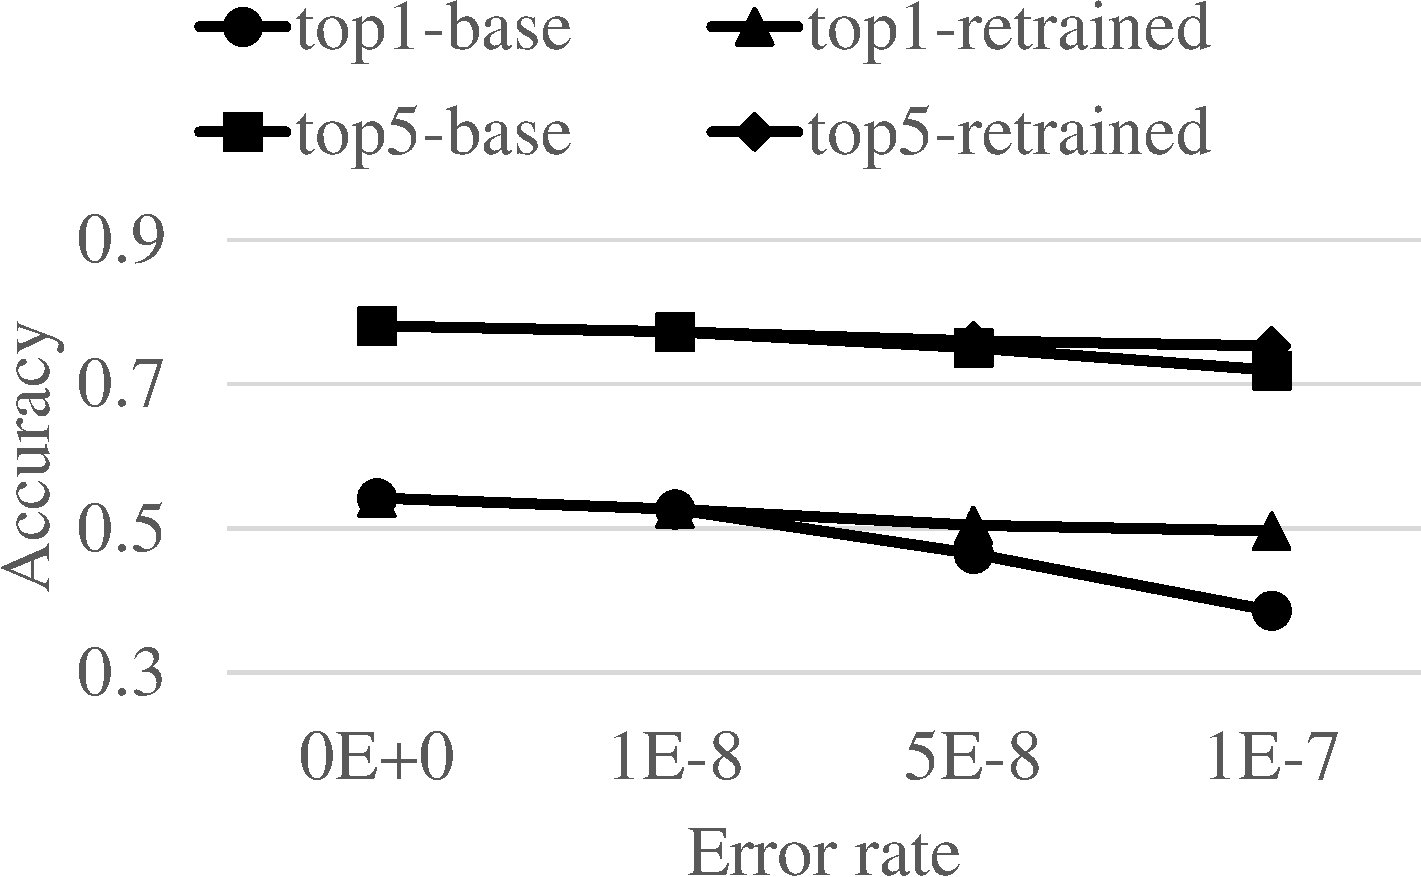
\includegraphics[width=0.7\linewidth]{alexnet-softerror}
        }
        \qquad
        \subfloat[VGG-16]{
                \label{fig:vgg16}
                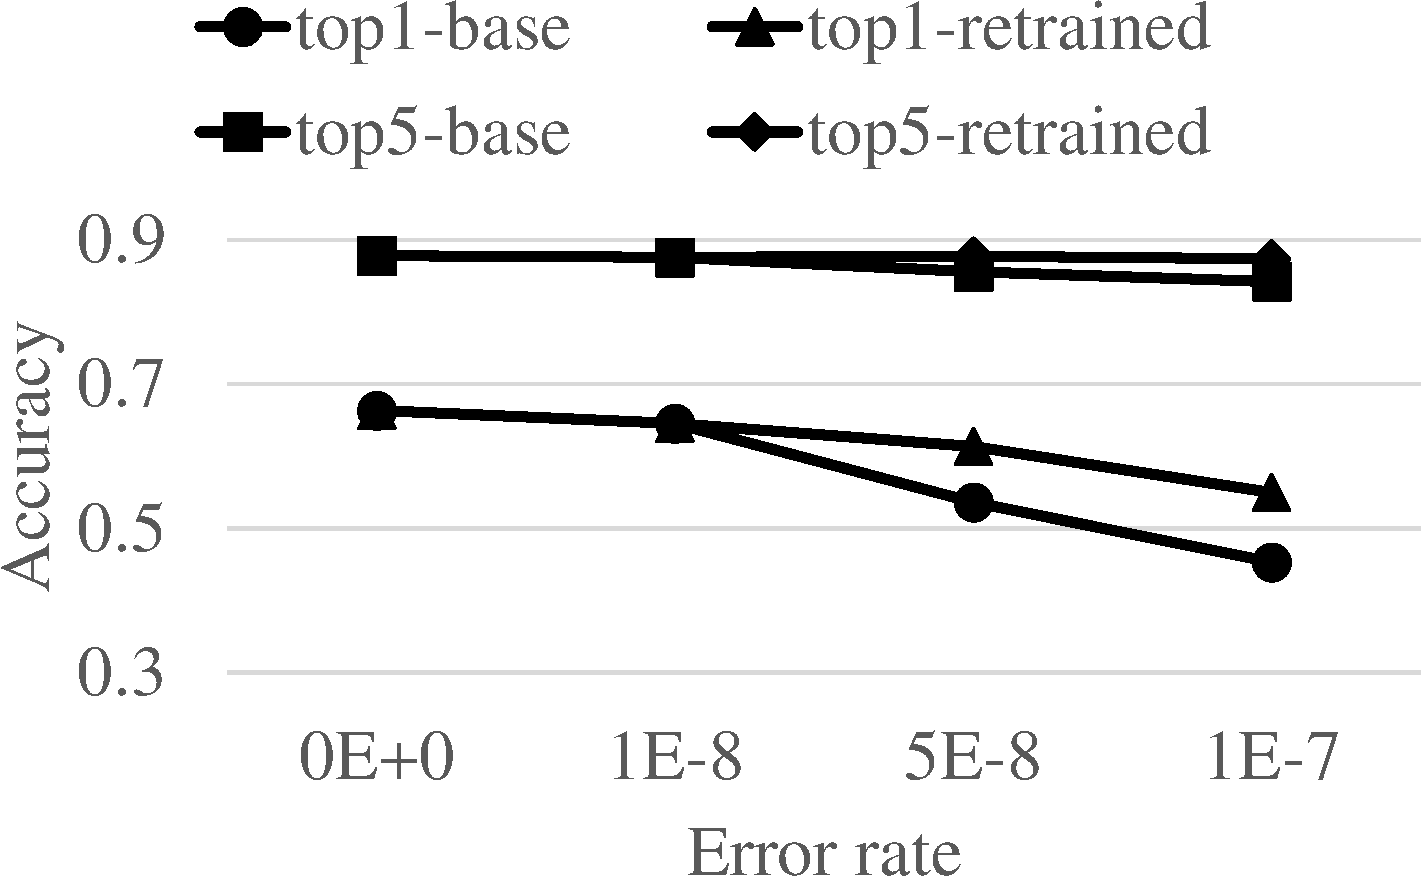
\includegraphics[width=0.7\linewidth]{vgg16-softerror}
        }
        \qquad
        \subfloat[VGG-19]{
                \label{fig:vgg19}
                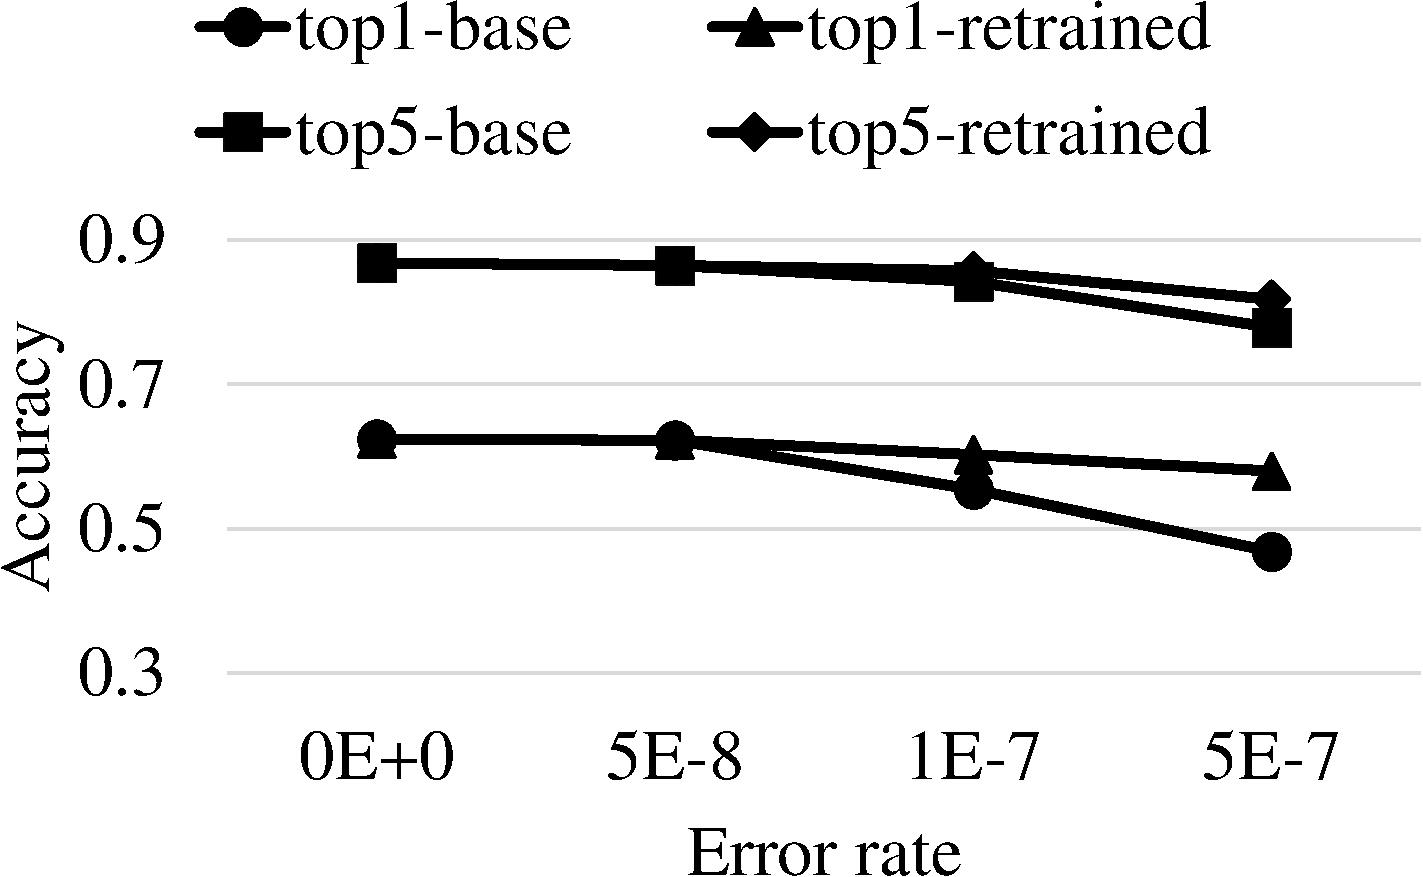
\includegraphics[width=0.7\linewidth]{vgg19-softerror}
        }
        \caption{The precision accuracy of the benchmark neural network models on accelerators with different computing errors}
        \label{fig:softerror-accuracy}
\end{figure}

\begin{figure}
        \center{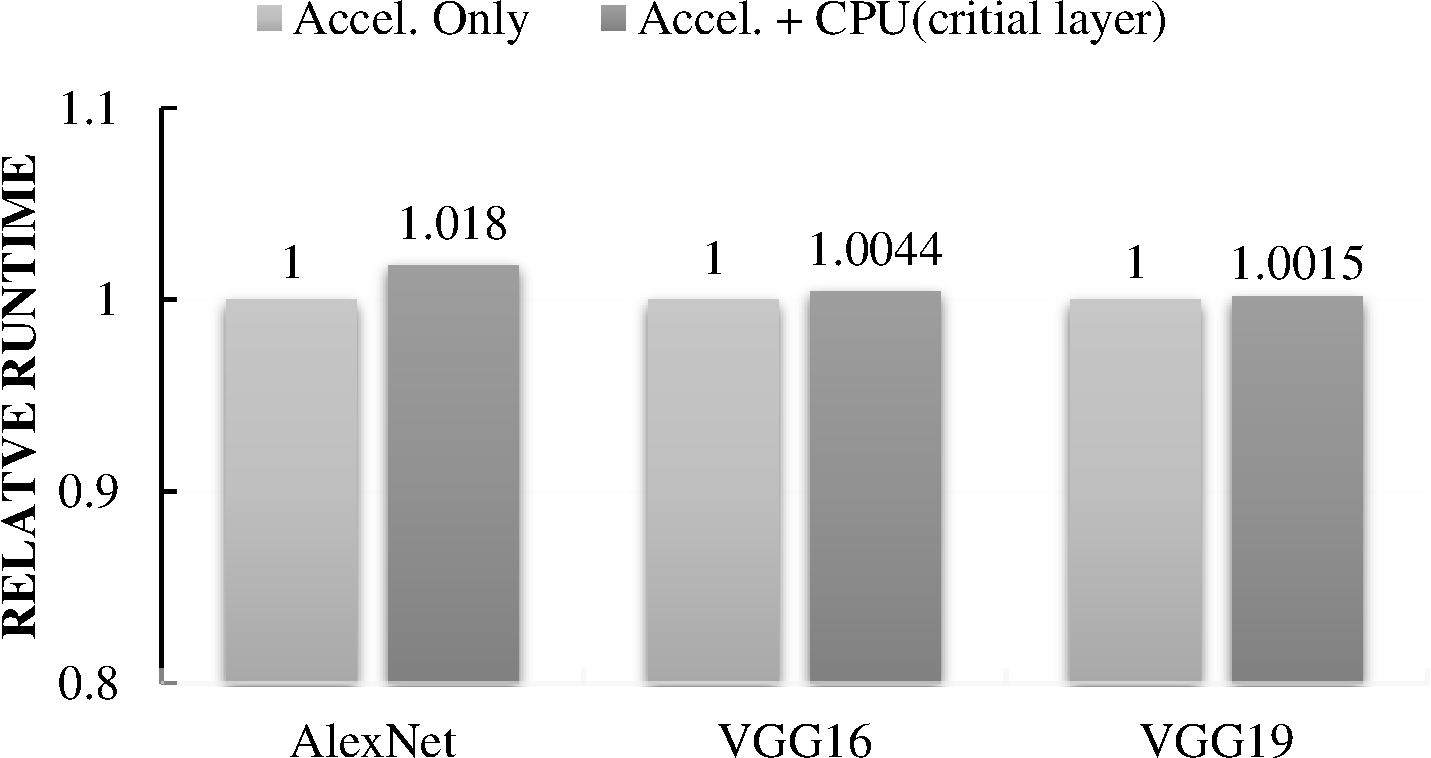
\includegraphics[width=0.7\linewidth]{clp_time}}
        \caption{Relative runtime of neural networks when the critical layer is scheduled to CPU.}
        \label{fig:clp_perf}
\end{figure}

We decide the critical layers using the error distribution as shown in Figure \ref{fig:clp_perf}.
We set the error threshold to be 5 and the experiment reveals that the last FC 
layer has the largest portion of computing errors that are more than 5. Thus, it is considered as 
the most critical layer. The critical layer takes only a small portion of the overall 
neural network computing, so the performance penalty is small even 
when it is scheduled to CPU. The last FC layer in AlexNet takes up higher portion of computing, 
the performance penalty is relatively higher compared to VGG16 and VGG19.
\begin{figure*}
        \center{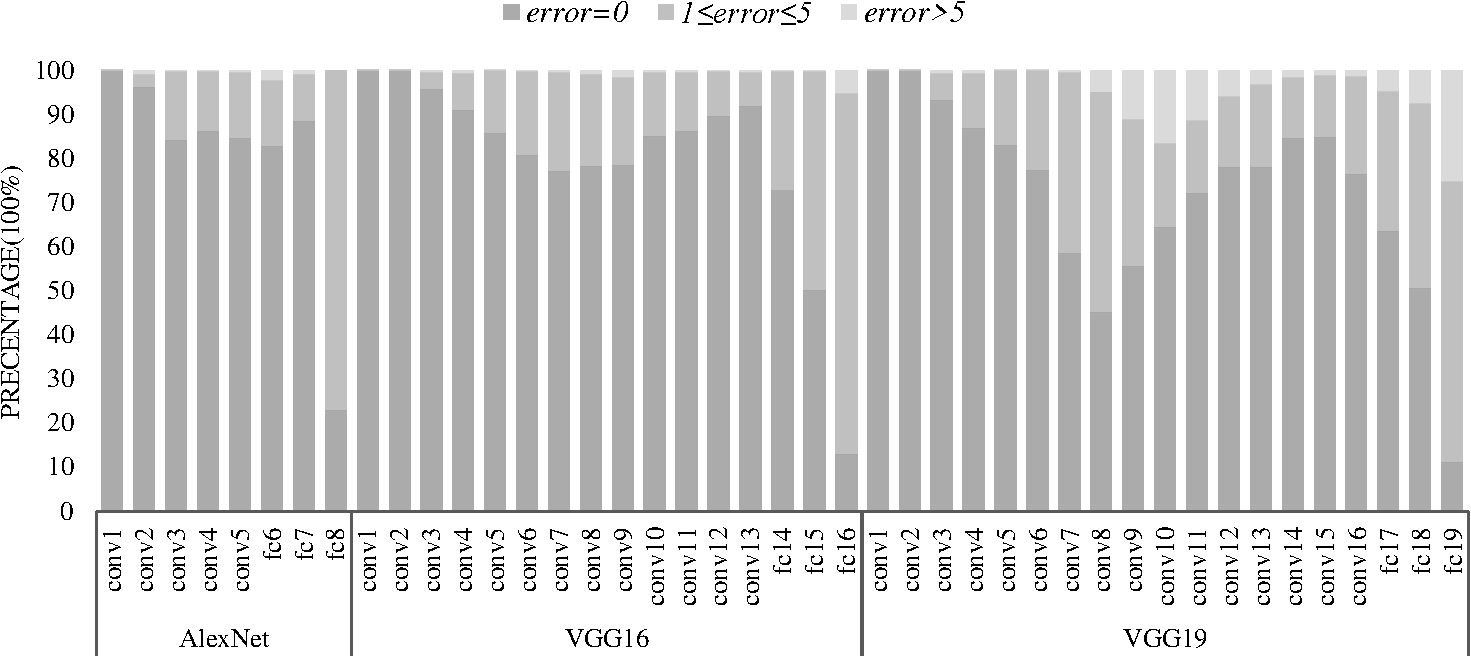
\includegraphics[width=0.8\linewidth]{error_distribute_softerror}}
        \caption{Error distribution across the neural network layers when highest BER is used in AlexNet, VGG16 and VGG19.}
        \label{fig:clp_perf}
\end{figure*}

\subsection{Overclocking case study}
To verify the proposed resilient training, we take overclocked CNN accelerator on KCU1500 as a case 
study in this work. By relaxing the timing constraints, the CNN accelerator can 
run at higher clock frequency with timing violations and computing errors. In PipeCNN, the 
hardware implementation is related to the neural network. For AlexNet, VGG16 and VGG19, the 
default implementation frequency is 210 MHz, 190 MHz and 190 MHz respectively. We then apply overclocking 
on the implementations with 10MHz step. The frequency can be boosted to 
260 MHz MHz, 240 MHz MHz and 240 MHz at most. By retraining the original neural network with 
the proposed approach, the prediction accuracy improvement is evaluated in detail.

With the overclocked CNN accelerators, we compare both the offline 
training and the proposed resilient training as presented in Figure \ref{fig:overclock-accuracy}. 
The prediction accuracy remains unchanged at the beginning and exhibits cliff-like drop 
at a tipping point. Beyond the tipping point, the prediction is no longer interesting 
due to the extremely low accuracy. At the tipping point, the top1 and top5 prediction accuracy of the 
retrained neural networks improves by xxx and xxx respectively.

\begin{figure}
        \center
	\subfloat[AlexNet]{
                \label{fig:alexnet}
                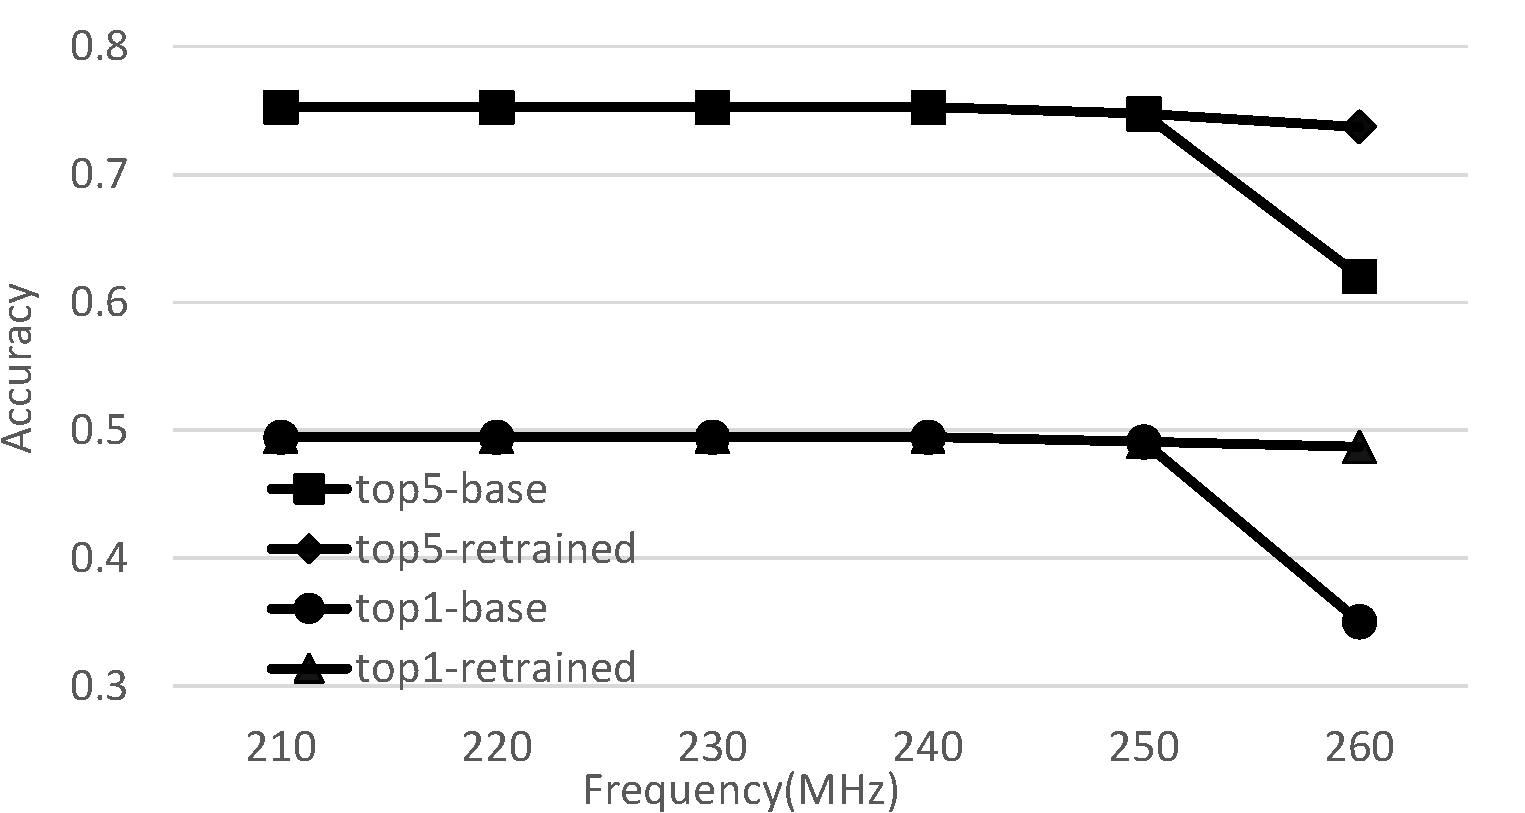
\includegraphics[width=0.6\linewidth]{alexnet-overclock}
        }
	\qquad
	\subfloat[VGG-16]{
                \label{fig:vgg16}
                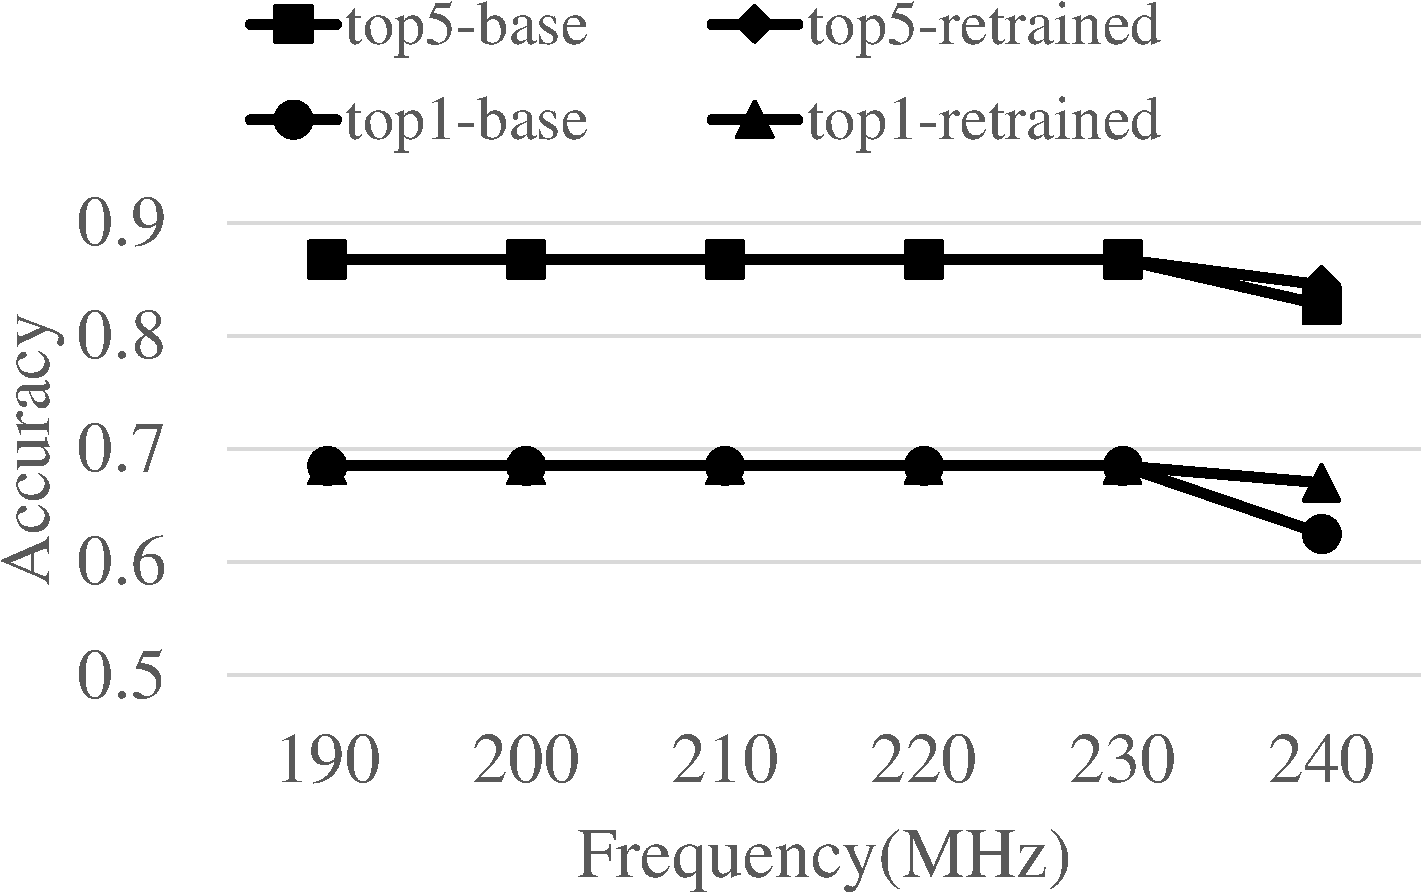
\includegraphics[width=0.6\linewidth]{vgg16-overclock}
        }
        \qquad
	\subfloat[VGG-19]{
                \label{fig:vgg19}
                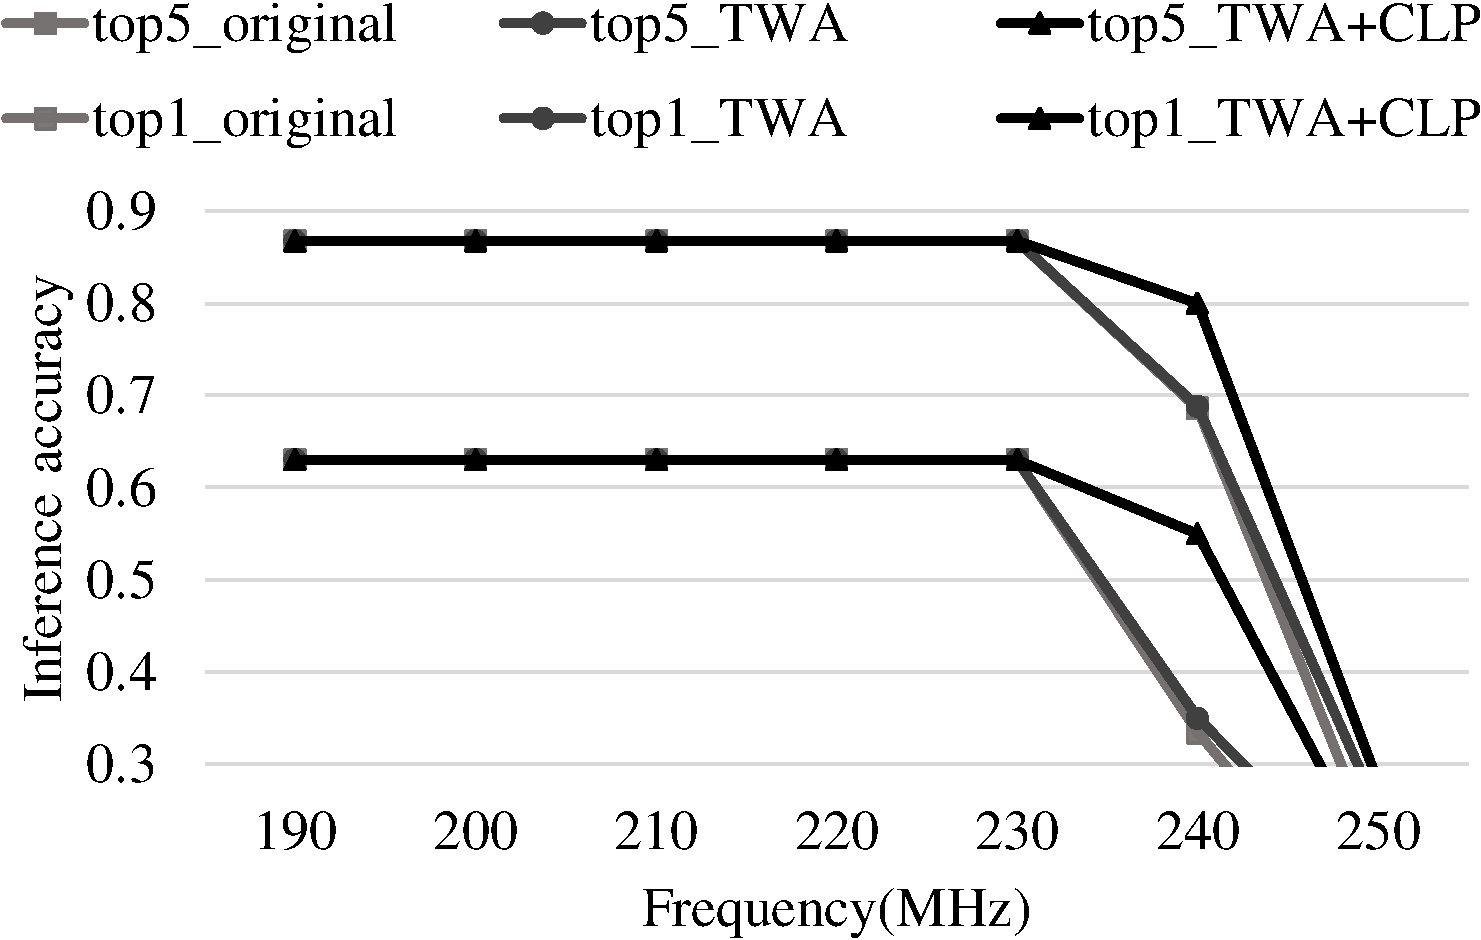
\includegraphics[width=0.6\linewidth]{vgg19-overclock}
        }
	\caption{The prediction accuracy of the benchmark neural networks on accelerators with different overclocking}
        \label{fig:overclock-accuracy}
\end{figure}

Clock frequency is almost proportional to the performance of the CNN accelerator 
especially for large convolution operation which is typically computing bound. 
Figure \ref{fig:overclocking-time} shows the relative inference runtime of the three neural networks at different 
overclocking. On the tipping point which is also the extreme overclocking case, 
the runtime improves by xxx compared to the models running on normal accelerator with 
xxx top1 accuracy loss and xxx top5 accuracy loss on average. 
\begin{figure}
        \center{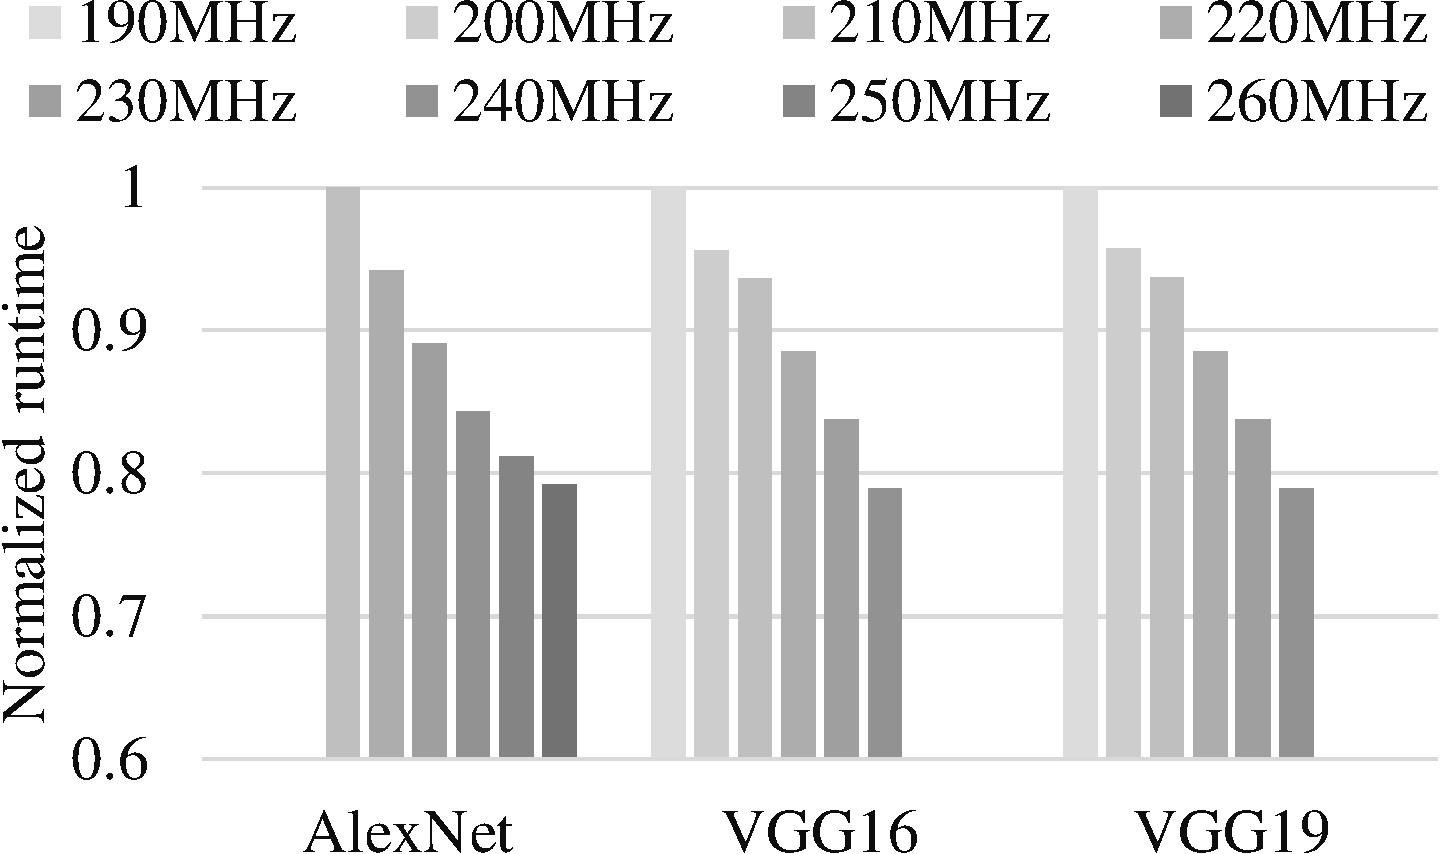
\includegraphics[width=0.6\linewidth]{relative-runtime}}
        \caption{Relative runtime of the neural networks on CNN accelerators with different overclocking. Note that AlexNet runs from 210 MHz to 250 MHz while 
		VGG16 and VGG19 ranges from 190 MHz to 240MHz, so some of the data is left blank.}
        \label{fig:overclocking-time}
\end{figure}

Comparing the experiments with random error simulation and overclocking on realistic FPGAs, we
find that the computing errors may not be uniformly distributed. In the overclocking,  
the prediction accuracy drops with cliff-like style. It indicates the computing errors may 
be quite small with light overclocking, but the amount of errors explodes at certain point.
Fortunately, the general trend is similar and the proposed training produces more resilient 
neural networks. 



%\section{Related Work} \label{sec:relatedwork}
Despite of the performance and power advantages, the design 
productivity of developing FPGA applications remains low 
due to the lengthy compilation and complex application-specific 
customization. And it has become the major obstacle 
that hinders the wide adoption of FPGAs as commodity computing devices. 
The community from both the industry and academia have developed 
many different methods from diverse angles to tackle the problem. 
These methods can be roughly classified into three categories. 
The first category mainly focuses on improving the low-level 
implementation tools. A number of approaches such as making 
quality/runtime trade-offs \cite{mulpuri2001runtime}, parallel 
compilation \cite{moctar2014parallel, goeders2011deterministic, altera-pc, 
xilinx-pc} and using hard-macro techniques \cite{lavin2013improving, 
korf2011automatic} have been explored from this angle. The second 
category mainly centers the HLS design flow while the third one 
primarily relies on the overlay concept. They later two categories 
will be detailed in the following sections.

\subsection{High-Level Synthesis} 
With many years of continuous endeavor, a number of tools have emerged as 
mature solutions for HLS \cite{VivadoHLS, Legup, zhang2008autopilot}. They typically 
allow designers to express hardware designs using high-level  
description languages such as C, C++ etc. and also enable evaluation of different 
design choices using pragmas or directives. Indeed, they significantly improve 
the design productivity compared to the conventional hardware design flow using 
hardware description languages. However, when considering the overall design 
productivity of developing hybrid software-gateware applications, HLS is 
only addressing part of the problem, as the lengthy low-level compilation 
including synthesis, mapping, placing and routing remains a bottleneck for 
an application designer \cite{ROB2014, capalija2014tile}.

Customizing the generated hardware specifically to an user 
application is also time-consuming for designers and thus critical to the design 
productivity. A number of algorithms such as generic algorithms 
relied on local-search techniques \cite{schafer2009adaptive, 
sengupta1997genetic}, learning-based methods \cite{onlinecustomization, 
carrion2012machine}, divide and conquer algorithm \cite{DCcustomization} 
and a calibration free algorithm \cite{RCcustomization} etc. have been developed 
to perform the DSE on top of HLS tools. The algorithms can efficiently help automate the 
customization or DSE process. However, the algorithms must rely on HLS tools 
to estimate the implementation information such as implementation frequency, 
overhead or power for the corresponding customization. While the hardware generated 
can be irregular and may vary dramatically, thus the accuracy of the estimation 
especially on implementation frequency and power can be rather limited, which may
fail to optimize an HW/SW co-design problem.  

\subsection{Overlay Architectures}
Overlay architecture which is a virtual intermediate architecture overlaid on 
top of off-the-shelf FPGA is increasingly applied as a way to address the 
productivity challenge. 

Various overlays with diverse configuration granularities and flexibility 
ranging from virtual FPGAs \cite{Grant2011Malibu, ZUMA2012}, 
array-of-FUs \cite{mesh-FUs,ferreira2011fpga}, soft 
CGRA \cite{kissler2006dynamically, scgra-orig}, soft GPU \cite{Guppy2012GPU-Like}, 
vector processors\cite{Yiannacouras2009FPS, MXP2013} to 
configurable processors or multi-core processors \cite{unnikrishnan2009application, 
MARC2010, Yiannacouras2007Exploration, Capalija2009coarse-grain, OCTAVO2012, iDEA2012} 
have been developed over the years. SCGRA overlay provides unique 
advantages on compromising hardware implementation 
and performance for compute intensive nested loops as demonstrated 
by numerous ASIC CGRAs \cite{tessier2001reconfigurable, compton2002reconfigurable}.
Most importantly, it allows both rapid compilation by taking advantage of 
the overlays' tiling structure \cite{ROB2014} and efficient bitstream 
reuse within the design iterations of an application \cite{scgra-orig}, 
thus it is particularly promising for high productivity nested loop acceleration.

Despite of the promising potential, a complete automatic customization 
framework that enables application-specific optimization is still highly 
anticipated for the sake of design productivity and performance. 
The authors in \cite{colinheart} developed an SCGRA topology customization method 
using genetic algorithm and showed the potential benefits of the SCGRA 
overlay customization. However, the rest system design parameters such as 
on chip buffer size, loop unrolling factor etc. are not covered. 

Indeed, SCGRA overlays have many similarities in terms of array structure 
and scheduling algorithm with ASIC CGRAs. Nevertheless, ASIC CGRAs emphasize 
more on configuration capability and limited customization is allowed due 
to the overhead constraints \cite{zhou2014application, miniskar2014retargetable} 
while SCGRA overlays allow more intensive architectural customization 
because of the FPGA's inherent programmability. Moreover, hardware resources such as 
DSP blocks and RAM blocks available on FPGAs are discrete, which results in different 
design constraints for SCGRA overlay customization as well. 

By utilizing the SCGRA overlay as the backbone of the FPGA accelerator, 
a complete nested loop acceleration framework 
targeting CPU-FPGA system is developed. It supports intensive application-specific
customization including the overlay architectural customization, 
the compilation customization and communication interface customization 
for various design goals. When the customized design parameters are determined, 
corresponding hardware accelerator and software can be compiled to the target 
CPU-FPGA system rapidly eventually providing a push-button solution for a nested loop 
acceleration. 



\section{Conclusion} \label{sec:Conclusion}
In this work, we propose to replace the forward computing on GPPs with accelerator 
computing during training and have both the computing 
errors and the application data learned in the neural network models. 
In addition, we opt to protect critical neural layers to reduce the negative 
influence of computing errors.  
With the proposed resilient neural network training, 
the prediction accuracy of the retrained neural network models improves significantly 
when computing errors appear. 


%\appendix
%\section{Acknowledgement}

%\begin{acks}
%  The authors would like to thank Sam Ho for providing the suggestions on
%  HLS design debugging and optimization as well as the SDAccel usage. 

%\end{acks}

\section*{Acknowledgement}
kkkkkkkkkkkkkkkkkkkkkkkkkkkkkkkkkkkkkkk
kkkkkkkkkkkkkkkkkkkkkkkkkkkkkkkkkkkkk
kkkkkkkkkkkkkkkkkkkkk


\bibliographystyle{IEEEtran}
\bibliography{refs} 




% trigger a \newpage just before the given reference
% number - used to balance the columns on the last page
% adjust value as needed - may need to be readjusted if
% the document is modified later
%\IEEEtriggeratref{8}
% The "triggered" command can be changed if desired:
%\IEEEtriggercmd{\enlargethispage{-5in}}

% references section

% can use a bibliography generated by BibTeX as a .bbl file
% BibTeX documentation can be easily obtained at:
% http://mirror.ctan.org/biblio/bibtex/contrib/doc/
% The IEEEtran BibTeX style support page is at:
% http://www.michaelshell.org/tex/ieeetran/bibtex/
%\bibliographystyle{IEEEtran}
% argument is your BibTeX string definitions and bibliography database(s)
%\bibliography{IEEEabrv,../bib/paper}
%
% <OR> manually copy in the resultant .bbl file
% set second argument of \begin to the number of references
% (used to reserve space for the reference number labels box)
%\begin{thebibliography}{1}

%\bibitem{IEEEhowto:kopka}
%H.~Kopka and P.~W. Daly, \emph{A Guide to \LaTeX}, 3rd~ed.\hskip 1em plus
%  0.5em minus 0.4em\relax Harlow, England: Addison-Wesley, 1999.

%\end{thebibliography}




% that's all folks
\end{document}



